\chapter{Realizzazione della soluzione}\label{chap:Realizzazione della soluzione}

\section{Introduzione}\label{chap:Introduzione}
Questo capitolo introduce i file e lo strumento Python sviluppati per estendere un file di tipo manifest Kubernetes, in modo da includere i componenti che dotano il cluster delle capacità di logging richieste.
È possibile applicare tutti i componenti tramite il comando:
\begin{lstlisting}[language=bash,label=lst:kubectl-apply,]
kubectl apply -f <file.yaml>
\end{lstlisting}
E in seguito, rimuovere il tutto tramite:
\begin{lstlisting}[language=bash]
kubectl delete -f <file.yaml>
\end{lstlisting}

Non si permette, infatti, nessuna esecuzione di script o codice arbitrario, in quanto non è possibile prevedere l'architettura del cluster di destinazione: l'unica interazione che si ha sul cluster è con i comandi suddetti.

L'implementazione della soluzione proposta si divide in due fasi: la prima riguarda l'ottenimento dei file necessari per dispiegare tutti i componenti che la costituiscono. Nella seconda fase, si passa invece all'implementazione del programma che modifica automaticamente un deployment per renderlo conforme all'obiettivo della tesi.

È possibile trovare il codice completo nella repository GitHub riportata di seguito.

\verb|https://github.com/belgio99/k8s-log-enabler|.

Sono inoltre presenti tutti i dispiegamenti utilizzati per la fase di validazione, tutti i log prodotti, e metriche dettagliate per l'analisi della latenza della soluzione proposta.


\section{Ottenimento e preparazione dei file necessari}\label{sect:Ottenimento e preparazione dei componenti}

\subsection{Creazione del file manifest di Istio}\label{subsec:Creazione del file manifest di Istio}
Per l'ottenimento di un file manifest \myenquote{vergine} di Istio da poter poi inserire nella repository del progetto, è stato usato lo strumento da riga di comando \verb|istioctl|\footnote{https://istio.io/latest/docs/reference/commands/istioctl/}. Questo strumento, infatti, è dotato di una funzionalità che permette la creazione di un file predefinito, in seguito applicabile ad un cluster Kubernetes non provvisto della suddetta utility installata.

Il comando necessario per la creazione del file è riportato nel Codice \ref{lst:istioctl_manifest_generate}.
\begin{lstlisting}[caption={Comando per la creazione del file manifest di Istio.}, label=lst:istioctl_manifest_generate]
istioctl manifest generate \\
-r logrevision \\
--set profile=minimal \\
--set meshConfig.accessLogFile=/dev/stdout  \\
--set meshConfig.accessLogFormat={...}  \\
--set meshConfig.accessLogEncoding=JSON  \\
--set namespace=log-istio-system \\
--set values.global.istioNamespace=log-istio-system \\
> istio_manifest.yaml
\end{lstlisting}

Scendendo nel dettaglio, il funzionamento di ogni parte del comando è descritto nella lista sottostante:
\begin{itemize}

\item \texttt{-r logrevision}: Opzione che specifica la revisione dell'installazione di Istio. La motivazione dettagliata di questa opzione è presente al Capitolo \ref{subsubsect:Uso delle revisioni di Istio}.

\item \texttt{--set profile=minimal}: Opzione che configura Istio utilizzando un profilo minimale, che installa solo il componente principale \verb|istiod|. Questo componente, infatti, è l'unico necessario per rendere possibile la funzione di access logging.
La lista completa di tutti i profili Istio è riportata in Figura \ref{fig:istio_profiles}:
\begin{figure}[h]
    \centering
    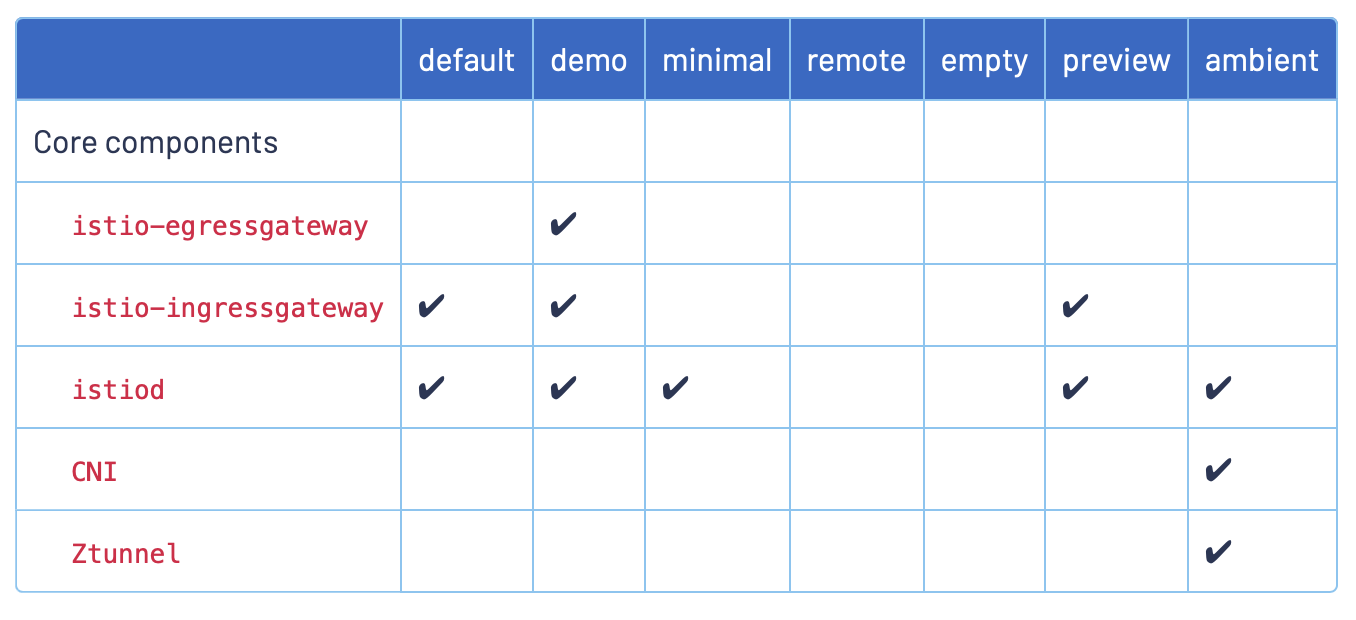
\includegraphics[width=1\linewidth]{immagini/capitolo4/istio_profiles.png}
    \caption{Tabella dei profili Istio disponibili \cite{istio_profiles}.}
    \label{fig:istio_profiles}
\end{figure}

\item \texttt{--set meshConfig.accessLogFile=/dev/stdout}: Parametro che redirige i file di log della rete mesh al flusso standard di output, in modo tale da essere poi direttamente raccolti da Filebeat senza ulteriori configurazioni.

\item \texttt{--set meshConfig.accessLogFormat=\{...\}}: Opzione che permette di definire un formato specifico per i log di accesso. Per brevità, nel comando soprastante questa parte è stata omessa, ma è disponibile nella sua interezza nel Codice \ref{lst:access_log_format}, presente al capitolo \ref{lst:access_log_format}.


\item \texttt{--set meshConfig.accessLogEncoding=JSON}: Determina il formato di codifica dei log di accesso. In questo caso, il formato è di tipo JSON, per rendere i log analizzabili da Logstash.

\item \texttt{--set namespace=log-istio-system}: Questo parametro specifica il namespace in cui Istio verrà installato. La scelta di un namespace dedicato, come \myenquote{log-istio-system}, è trattata al Capitolo \ref{sect:Spostamento delle risorse in namespace dedicati}.

\item \texttt{--set values.global.istioNamespace=log-istio-system}: Parametro che modifica un valore specifico all'interno del file di configurazione di Istio, per specificare il namespace nel quale deve cercare il suo \textit{control plane}.

\item \texttt{> istio\_manifest.yaml}: Questa parte finale del comando redirige l'output del comando precedente, ovvero il manifest generato, in un file chiamato \myenquote{istio\_manifest.yaml}, invece di stamparlo a schermo.

\end{itemize}

\subsection{Precauzioni adottate per evitare conflitti}

Nonostante il comando riportato nel paragrafo \ref{subsec:Creazione del file manifest di Istio} generi un file \verb|yaml| conforme alle specifiche di Istio per il deployment dello stesso senza \verb|istioctl|, è stato necessario prendere ulteriori precauzioni per evitare qualsiasi possibile conflitto con deployment già presente sul cluster.

Infatti, nonostante la creazione di namespace separi il più possibile le risorse, alcune di esse sono globali (dette anche \myenquote{\textit{cluster-wide}}) e possono interferire o essere interferite da risorse simili esistenti nel cluster. A causa di ciò, è necessario assicurarsi che ogni componente del file manifest di Istio sia adeguatamente configurato per evitare conflitti e rispettare le specifiche del progetto.

In particolare, sono state necessarie le seguenti modifiche:

\subsubsection{Uso delle revisioni di Istio}\label{subsubsect:Uso delle revisioni di Istio}
Negli ambienti dove può essere presente più di un control plane di Istio, è necessario un sistema di separazione ulteriore a quello provvisto dai namespace. Infatti, la separazione creata da questi ultimi non è sufficiente a garantire un isolamento completo dei control plane di Istio, visto il funzionamento inter-namespace del sistema. Per far fronte a questa necessità, gli sviluppatori di Istio mettono a disposizione il concetto di \textbf{revisione}: questa caratteristica può essere utilizzata per gli upgrade o per sperimentare con diverse configurazioni di Istio, senza influenzare il funzionamento globale. Ogni revisione di Istio viene identificata da un'etichetta unica, garantendo che le risorse siano separate e che non entrino in conflitto l'una con l'altra \textit{(Figura \ref{fig:revs})}.

\begin{figure}[h]
    \centering
    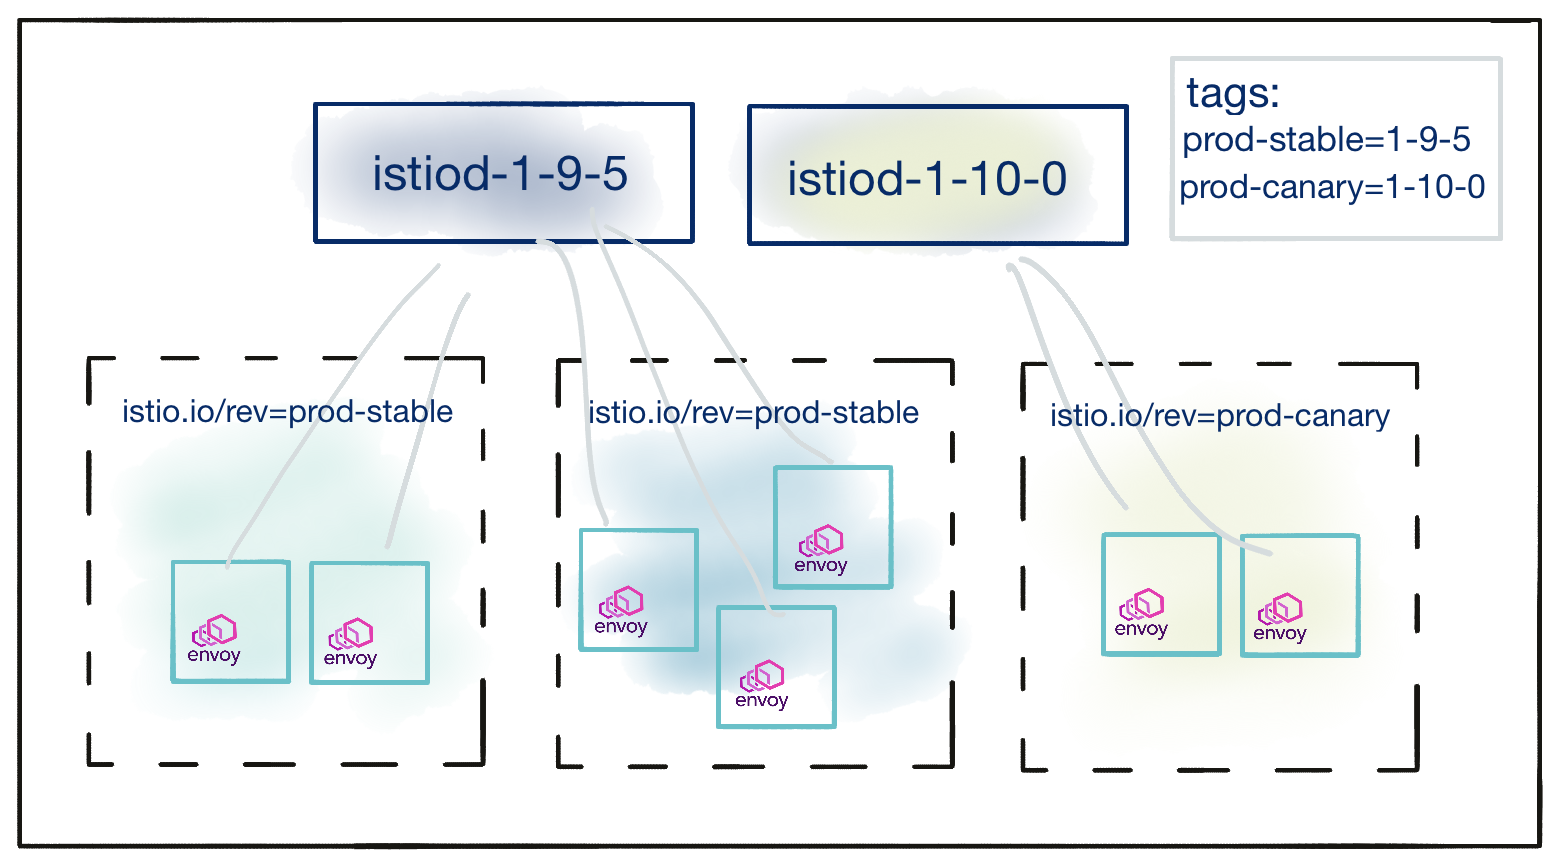
\includegraphics[width=\textwidth]{immagini/capitolo4/tags.png}
    \caption{Utilizzo tipico delle revisioni di Istio \cite{istio_revisions}.}
    \label{fig:revs}
\end{figure}



Nel contesto di questo progetto, l'utilizzo delle revisioni rende impossibile il verificarsi di una doppia iniezione del sidecar Envoy (la versione fornita nel progetto, e la versione eventualmente già presente in un cluster), in quanto l'iniezione segue queste precise regole:
\begin{itemize}
\item La revisione del control plane deve corrispondere con l'etichetta della revisione nel namespace (o nel pod) per cui si sta richiedendo l'iniezione.
\item Se nel namespace esistono più etichette di revisione, verrà utilizzata quella specificata nel pod. Se non è specificata alcuna etichetta nel pod, Istio non inietterà il sidecar.
\item Se non esiste alcuna etichetta di revisione nel namespace o nel pod, verrà utilizzato il control plane di default (se presente), ovvero il control plane che non possiede alcuna etichetta di revisione. Se quest'ultimo non è presente, l'iniezione non verrà effettuata.
\end{itemize}

Nel caso specifico, è stata utilizzata l'opzione \texttt{-r logrevision} nel comando di creazione del manifest per assegnare una revisione alla versione di Istio fornita nel progetto, come menzionato nella sezione precedente. Questa revisione consente di identificare e distinguere l'installazione di Istio dedicata alla funzione di access logging dalle altre potenziali installazioni di Istio presenti nel cluster.

Di conseguenza, è stata applicata l'etichetta \verb|istio.io/rev: logrevision| al namespace \verb|log-enabled|, per poter consentire alla versione di Istio fornita nel progetto l'iniezione del sidecar Envoy configurato per l'access logging solo su tale namespace.

\subsubsection{Separazione delle estensioni CustomResourceDefinitions}
Le \textit{CustomResourceDefinitions} (CRD) in Kubernetes sono estensioni dell'API che consentono di definire tipi di risorse personalizzate. Istio si avvale delle CRD per definire e configurare vari componenti che non rientrano nelle risorse native di Kubernetes.

Poiché le CRD sono globali all'interno di un cluster Kubernetes, esiste un rischio concreto di conflitto con altre installazioni di Istio se le definizioni fornite nel progetto interferiscono con CRD già esistenti, specialmente durante il processo di eliminazione delle risorse. Di conseguenza, si è deciso di adottare delle precauzioni nella gestione delle CRD di Istio.

Entrando più nel dettaglio, il comando spiegato alla sezione \ref{subsec:Creazione del file manifest di Istio} crea automaticamente un unico file contenente sia CRD che componenti di Istio. Dato che l'obiettivo è invece quello di poter condividere il cluster con eventuali componenti Istio già presenti, un'eventuale eliminazione delle CRD di Istio comprometterebbe il funzionamento dei componenti in esecuzione sugli altri namespace (come ad esempio il predefinito \verb|istio-system|).

Separando quindi CRD e componenti, qualora fosse già in esecuzione un'installazione di Istio in un altro namespace, è possibile saltare il passaggio di applicazione delle CRD.

\subsection{Creazione del file manifest per lo stack ELK}\label{reazione del file manifest per lo stack ELK}
Per la creazione del file manifest dello stack ELK, che è stato appositamente realizzato e configurato per questo scopo, sono stati necessari i seguenti componenti:
\begin{itemize}
\item \textbf{ServiceAccount, ClusterRole, e ClusterRoleBinding:} Componenti che forniscono a Filebeat le possibilità di interagire con le API di Kubernetes. In questo modo, è possibile arricchire i log con metadati di Kubernetes come namespace e nome del pod.

\item \textbf{Configmap:} Componenti contenenti i file di configurazione delle applicazioni Logstash e Filebeat.

\item \textbf{StatefulSet per ElasticSearch:} Componente che permette di mantenere uno stato consistente tra varie istanze di ElasticSearch. Ciò garantisce che ogni pod abbia un identificatore unico, rendendo possibile la scalabilità orizzontale del cluster in futuro.

\item \textbf{Deployment per Logstash, Kibana e Filebeat:} Per queste componenti non è necessario mantenere uno stato persistente tra le distribuzioni. Pertanto, è stato utilizzato un Deployment per gestire la loro distribuzione e scalabilità.

\item \textbf{Servizi:} I servizi per ElasticSearch, Logstash e Kibana sono necessari per permettere la comunicazione tra i componenti e l'accesso ai servizi da parte di altre applicazioni o utenti.

\item \textbf{DaemonSet per Filebeat:} Componente che assicura l'esecuzione di Filebeat su ogni nodo del cluster. Questo permette a Filebeat di catturare tutti i log da tutti i nodi.

\item \textbf{Volume e VolumeMounts:} Componenti utilizzati per fornire spazio di archiviazione persistente per ElasticSearch e per permettere a Filebeat di accedere ai log dei container.

\end{itemize}

\subsection{Creazione dei namespace dedicati}
Come riportato nel Capitolo \ref{sect:Spostamento delle risorse in namespace dedicati}, è stata progettata la creazione di tre nuovi namespace per separare le risorse e garantire un'organizzazione ottimale delle componenti nel cluster.

Per la creazione dei namespace, è stato aggiunto nella parte iniziale dei file l'apposito codice YAML, con le eventuali label già predisposte. Ad esempio, per il namespace \verb|log-enabled|, è stato sviluppato lo snippet del codice \ref{lst:log-enabled-creation}. In tale snippet, è possibile anche individuare la parte relativa all'etichettatura con la revisione di Istio fornita nel progetto:
\begin{lstlisting}[caption={Snippet della creazione del namespace log-enabled},label=lst:log-enabled-creation, escapechar=|]
apiVersion: v1
kind: Namespace
metadata:
  name: log-enabled
  labels:
    istio.io/rev: logrevision
\end{lstlisting}


\section{Script Python: introduzione e funzionalità di iniezione dei componenti}

Una volta ottenuti i file principali trattati dal capitolo \ref{sect:Ottenimento e preparazione dei componenti}, usati dallo script Python come sorgenti per la creazione del file .yaml finale, è necessario applicare delle piccole modifiche al deployment originale in modo che possa funzionare come richiesto. Nei paragrafi successivi, viene trattato il funzionamento dello script.

\subsection{Organizzazione dei file di progetto}
Il progetto Python è diviso in più file e cartelle:
\paragraph{Cartella radice}
\begin{itemize}
    \item \texttt{main.py:} File principale del progetto, contenente le funzioni di iniezione e di connessione ad ElasticSearch.
    \item \texttt{yrca.py:} File contenente le funzioni relative all'elaborazione di log per il formato richiesto da yRCA.
    \item \texttt{utils.py:} File contenente alcune funzioni di utilità, inserite in questo file per garantire una migliore organizzazione del codice.
    \item \texttt{requirements.txt:} File contenente tutti i moduli richiesti dal progetto, ed installabili tramite \textit{pip}.
\end{itemize}
\paragraph{Cartella \myenquote{manifest}}
\begin{itemize}
    \item \texttt{istio\_manifest.yaml:} File contenente il manifest \texttt{.yaml} di Istio, trattato nel Capitolo \ref{subsec:Creazione del file manifest di Istio}.
    \item \texttt{elk\_manifest.yaml:} File contenente il manifest \texttt{.yaml} dello stack ELK, trattato nel Capitolo \ref{reazione del file manifest per lo stack ELK}.
    \item \texttt{namespace\_manifest.yaml:} File contenente il file manifest \texttt{.yaml} relativo alla creazione del namespace che conterrà il deployment di cui ottenere i log.
\end{itemize}

\subsection{Moduli e librerie usate}
Per la stesura dello script, si sono usati i seguenti moduli e librerie:
\begin{itemize}
    \item \textit{Argparse:} Modulo della libreria standard di Python \cite{python_standard_library}, usato per facilitare la scrittura a riga di comando. Oltre alla possibilità di poter accedere ai parametri passati via riga di comando in modo molto intuitivo, include la possibilità di scrivere un \textit{help} in modo tale da guidare l'utente nella creazione del proprio comando.
    
    \item \textit{PyYaml:} Libreria esterna, inclusa per il supporto del linguaggio yaml, utilizzato da Kubernetes per il dispiegamento dei componenti.
    
    \item \textit{Elasticsearch:} Libreria esterna, aggiunta per comunicare con le API di ElasticSearch.
    
    \item \textit{Json:} Modulo standard Python che facilita l'elaborazione di file in formato JSON.
    
    \item \textit{Datetime:} Modulo standard Python che fornisce classi per manipolare date e orari. Offre funzioni per analizzare stringhe di date/tempo, fare aritmetica di date e formattare le date per la visualizzazione.
\end{itemize}

\subsection{Argomenti supportati dalla linea di comando}
Gli argomenti supportati dalla linea di comando sono:

\begin{itemize}

\item \texttt{-i, --inject} \textit{input\_file}: Inietta componenti di analisi del log nel file di input specificato.
    
\item \texttt{-o, --output}: Specifica un percorso di file di output personalizzato. Se non specificato, l'output del programma viene sempre stampato su \texttt{stdout}.

\item \texttt{-t, --timeout}: Specifica un timeout Envoy personalizzato. Se non specificato, il default è \myenquote{1m}.

\item \texttt{--no-header}: Permette di non aggiungere Istio e lo stack ELK al file di output finale. Opzione utile quando si vuole processare più file di deployment, dove basta che il primo file abbia i componenti suddetti, e non anche gli altri.

\item \texttt{-n namespace}: Permette di aggiungere un suffisso personalizzato al nome del namespace di destinazione, per consentire l'esecuzione di più applicazioni monitorabili contemporaneamente. Il nome finale del namespace risulterà quindi del tipo \texttt{log-enabled-suffisso}.

\item \texttt{-c, --connect} \textit{ElasticSearch\_instance}: Connette all'istanza di ElasticSearch specificata.

\item \texttt{-p, --port}: Specifica la porta di ElasticSearch. Il valore di default è 9200.

\item \texttt{--pod}: Scarica, dall'istanza di ElasticSearch, i log di un preciso pod (su un file, se utilizzato con -o). Non può essere utilizzato con il formato di output di log yRCA, in quanto quest'ultimo necessita esclusivamente dei log dei proxy Envoy.

\item \texttt{--dump-all}: Scarica, dall'istanza di ElasticSearch, i log di tutti i pod presenti nel namespace (su un file, se utilizzato con -o). Per la stessa motivazione del punto sopra, non può essere utilizzato con il formato di output di log yRCA.

\item \texttt{-f, --format}: Specifica il formato di output dei log. Le opzioni disponibili sono \texttt{yrca}, \texttt{gelf}, e \texttt{syslog}. Il valore predefinito è \texttt{yrca}.
\end{itemize}



\subsection{Processo di iniezione del file}
Il processo di modifica ed iniezione del file con tutti i componenti trattati nei paragrafi precedenti, avviene come segue:
\begin{enumerate}
    \item \textbf{Sostituzione del namespace di origine:} La prima azione che viene eseguita dallo script è quella introdotta nel Capitolo \ref{sect:Spostamento delle risorse in namespace dedicati}, ovvero la sostituzione del namespace di origine con il namespace dedicato alla raccolta e l'analisi di log \verb|log-enabled| (o, se specificato nel comando, \verb|log-enabled-suffisso|). Questo consente di ottenere il meccanismo di separazione dalle altre risorse nel cluster trattato nel Capitolo \ref{sect:Spostamento delle risorse in namespace dedicati}.


\item \textbf{Aggiunta degli Istio VirtualServices:}
Viene eseguito un parsing dedicato unicamente ai servizi presenti nel file di deployment, e per questi ultimi viene creato un Istio VirtualService, componente trattato nel capitolo \ref{subsect:Istio Virtual Service}, ed aggiunto in coda al file. Il componente sarà correttamente configurato con il timeout impostato dall'opzione \texttt{-t}.

\item \textbf{Unificazione dei file:}
Come ultimo passaggio, tutti i componenti menzionati vengono unificati in un solo file, in quest'ordine:
\begin{enumerate}
    \item Componenti di Istio
    \item Componenti dello stack ELK
    \item Dispiegamento da analizzare
    \item Istio VirtualServices
\end{enumerate}
\end{enumerate}

\section{Script Python: funzionalità di connessione all'istanza ElasticSearch}
La funzionalità di connessione all'istanza ElasticSearch è resa possibile tramite l'uso della libreria ElasticSearch di Python. Questa libreria fornisce un'interfaccia client di basso livello per interagire con un'istanza di ElasticSearch, per facilitare l'operazione di ricerca dei documenti.

Il funzionamento delle API di ElasticSearch è basato su un sistema di \textit{query}: per ottenere i dati desiderati, è necessario formare la query, ed inviarla tramite la funzione \texttt{connect}.

Per utilizzare le funzionalità di connessione a ElasticSearch, è stata creata nello script Python un'interfaccia che permette tre opzioni:
\begin{itemize}
    \item Lo scaricamento dei log relativi unicamente ai proxy Envoy (comportamento predefinito).
    \item Lo scaricamento dei log di un pod specifico (tramite l'opzione \texttt{--pod}).
    \item Lo scaricamento dei log di tutti i pod contenuti nel namespace \verb|log-enabled| (tramite l'opzione \texttt{--dump-all}).
\end{itemize}

\subsection{Utilizzo di ElasticSearch Scroll API per l'ottenimento dei dati}
Nell'utilizzo del programma Python, possono verificarsi casi in cui i log da scaricare possano superare un limite predefinito da ElasticSearch. Quest'ultimo, infatti, può fornire al massimo 10000 documenti per singola richiesta. Per far fronte alla possibilità che, in grandi deployment, possano essere prodotti più di 10000 documenti, si è optato per l'utilizzo della cosiddetta Scroll API \cite{scroll_api}. Il funzionamento è il seguente:
\begin{enumerate}
\item Inizialmente, viene eseguita una richiesta di ricerca a ElasticSearch specificando il parametro \textit{scroll}. Questo parametro indica la durata per la quale la ricerca sarà disponibile per lo scorrimento, permettendo così di ottenere più documenti in successione. In questa implementazione, il tempo di scorrimento è bloccato a 1 minuto.
\item La prima risposta, contenente la prima parte di documenti, includerà inoltre un ID di scroll. Quest'ultimo dovrà essere utilizzato nelle richieste successive per ottenere ulteriori documenti.

\item Continuando con questo meccanismo, è possibile ottenere tutti i documenti desiderati, superando il limite di 10000 documenti per singola richiesta. È fondamentale assicurarsi di proseguire con le richieste entro il periodo di tempo definito dal parametro \textit{scroll}, altrimenti la sessione si chiuderà, e sarà necessario iniziare nuovamente la richiesta.

\item Una volta ottenuti tutti i documenti necessari, è consigliabile chiudere la sessione di scroll utilizzando l'ID di scroll, per liberare le risorse utilizzate dalla richiesta sull'istanza ElasticSearch.

\end{enumerate}

\section{Script Python: funzionalità di esportazione dati}

Una volta che i dati sono stati ottenuti tramite l'ElasticSearch Scroll API, è necessario un post-processing per renderli disponibili nel formato desiderato all'avvio del programma.
I formati disponibili per l'esportazione dei dati sono tre:
\subsection{Formato yRCA}
Il formato di input per yRCA prevede 6 tipi di messaggi differenti. Questo formato richiede e necessita unicamente dei log dei proxy Envoy.
Il formato comprende sei tipi di messaggio, i quali sono descritti brevemente nella lista sottostante:
\begin{enumerate}
    \item \textbf{Invio della richiesta, lato client:} Prima dell'effettivo invio della richiesta, verrà emesso questo messaggio: \newline
    \texttt{"Sending message to [Other Service Name] (request\_id:[RequestId])"}

    \item \textbf{Ricezione di un messaggio, lato server:} Immediatamente dopo la ricezione della richiesta, verrà emesso questo messaggio: \newline
    \texttt{"Received POST request from [Other Service Name] (request\_id:[RequestId])"}

    \item \textbf{Invio della risposta, lato server:} Dopo l'elaborazione della richiesta e prima dell'invio della risposta (durante questo intervallo potrebbero verificarsi altre richieste), verrà emesso questo messaggio: \newline
    \texttt{"Answered to POST request from [Other Service Name] with code [Status Code] (request\_id:[RequestId])"}

    \item \textbf{Ricezione di una risposta OK, lato client:} Dopo aver ricevuto una risposta positiva, verrà emesso questo messaggio: \newline
    \texttt{"Receiving answer from [Other Service Name] (request\_id:[RequestId])"}

    \item \textbf{Ricezione di una risposta d'errore, lato client:} Nel caso in cui la risposta indichi un errore, verrà emesso questo messaggio: \newline
    \texttt{"Error response (code: [Response Code]) received from [Other Service Name] (request\_id:[RequestId])"}

    \item \textbf{Timeout expiration, lato client:} Se si verifica un errore dovuto a un timeout, verrà emesso questo messaggio: \newline
    \texttt{"Failing to contact [Other Service Name] (request\_id:[RequestId]). Root cause: [Root cause]"}
\end{enumerate}

Per potersi integrare con yRCA senza richiedere nessun processing esterno, questi sei tipi di output devono rispettare il formato di input richiesto da yRCA. Per fare ciò, i log vengono inseriti in un messaggio JSON contenente i seguenti campi:
\begin{itemize}
    \item \texttt{Severity:} la Severity dei log viene automaticamente applicata in base al tipo di messaggio di output. In particolare, questa è sempre impostata su INFO, tranne per quando vengono generati i messaggi di tipo 5 e 6 nella lista soprastante. In tal caso, la severity viene impostata su ERROR.
    \item \texttt{container\_name:} Il nome del pod che ha generato il messaggio.
    \item \texttt{event:} Uno dei sei tipi di messaggio descritti.
    \item \texttt{@timestamp:} La data e l'ora della generazione della linea, in formato ISO 8601.
    \item \texttt{timestamp:} La data e l'ora della generazione della linea, in formato ISO 8601, ma con separatori differenti.
    
\end{itemize}

In Figura \ref{lst:yrca-code}, è possibile vedere un messaggio di esempio che rispetta formato di output suddetto.

\begin{lstlisting}[caption={Formato di output per yRCA.},label=lst:yrca-code, escapechar=|, keywordstyle=\color{black}, commentstyle=\color{black},stringstyle=\color{black},numberstyle=\color{black}]
    {
    "severity": "ERROR", 
    "container_name": "k8s_checkoutservice", 
    "event": "Failing to contact paymentservice:50051 (request_id: [b7c3e034-e5a4-4797-af9a-2f66251ec6bc]). Root cause: ",
    "message": "2023-09-24 21:34:36.697 ERROR k8s_checkoutservice --- Failing to contact paymentservice:50051 (request_id: [b7c3e034-e5a4-4797-af9a-2f66251ec6bc]). Root cause: ",
    "timestamp": "2023-09-24 21:34:36.697",
    "@timestamp": "2023-09-24T21:34:36.697Z"
    }

\end{lstlisting}

\subsection{Formato GELF}

Il formato GELF (\textit{Graylog Extended Log Format}) \cite{gelf_format} è un formato di log progettato specificamente per il sistema di logging Graylog. È stato creato per superare le limitazioni dei formati dei log tradizionali consentendo un messaggio più strutturato e leggibile, grazie al formato JSON usato per specificare campi e valori.

GELF include campi standardizzati, ma può anche essere esteso con campi personalizzati in base alle esigenze. È riportato un esempio di un messaggio di log in formato GELF:

\begin{lstlisting}[caption={Esempio di messaggio in formato GELF.},label=lst:gelf-code, escapechar=|, keywordstyle=\color{black}, commentstyle=\color{black},stringstyle=\color{black},numberstyle=\color{black}]
{
  "version": "1.1",
  "host": "example.org",
  "short_message": "A short message",
  "full_message": "Backtrace here\n\nmore log informations",
  "timestamp": 1385053862.3072,
  "level": 1,
  "_user_defined_field": "user_defined_value"
}
\end{lstlisting}

Dove:

\begin{itemize}
  \item \texttt{version}: La versione del formato GELF.
  \item \texttt{host}: Il nome host o indirizzo IP del mittente.
  \item \texttt{short\_message}: Un breve messaggio descrittivo dell'evento. È obbligatorio e deve essere una stringa non vuota.
  \item \texttt{full\_message}: Un messaggio dettagliato o un backtrace, opzionale.
  \item \texttt{timestamp}: Il timestamp dell'evento, in secondi dal 1970-01-01T00:00:00Z.
  \item \texttt{level}: Il livello del messaggio, ad esempio 1 per \myenquote{alert} o 6 per \myenquote{info}.
  \item \texttt{\_campo\_personalizzato}: Qualsiasi campo aggiuntivo prefissato da un underscore (\_) è un campo personalizzato.
\end{itemize}

È importante notare che, mentre molti campi sono opzionali, GELF richiede almeno un \texttt{short\_message}. Se non si dispone di un valore utile, il valore \texttt{undefined} può essere utilizzato. I campi personalizzati possono invece essere utilizzati per arricchire i messaggi di log con informazioni specifiche del contesto, rendendo i dati di log più significativi. Nel progetto, infatti, sono stati aggiunti tre campi opzionali:
\begin{itemize}
    \item \texttt{\_namespace\_name}: Campo utilizzato per memorizzare il namespace del pod che ha generato la linea di log.
    \item \texttt{\_pod\_name}: Campo utilizzato per memorizzare il nome del pod che ha generato la linea di log.
    \item \texttt{\_container\_name}: Campo utilizzato per memorizzare il nome del container che ha generato la linea di log.
    
\end{itemize}


\subsection{Formato SYSLOG} SYSLOG \cite{gerhards_syslog_protocol} è un protocollo standard per l'invio di messaggi di log da dispositivi alla stazione di logging. Originariamente sviluppato negli anni '80, è diventato lo standard de facto per la registrazione di messaggi su Linux e su molte altre piattaforme. La struttura di un messaggio SYSLOG consiste in un header (che contiene informazioni come la data, l'ora e la sorgente del messaggio) seguito dal contenuto effettivo del messaggio.

Un messaggio SYSLOG si compone tipicamente delle seguenti parti:

\begin{itemize}
  \item \texttt{PRI}: Un numero che rappresenta la combinazione di facility e livello del messaggio. È una cifra che determina la priorità del messaggio.
  \item \texttt{HEADER}: Contiene due campi - il TIMESTAMP e il HOSTNAME del dispositivo o dell'applicazione che invia il messaggio.
  \item \texttt{MSG}: Il corpo del messaggio, che dettaglia l'evento o la situazione segnalata.
\end{itemize}

Un esempio di messaggio SYSLOG potrebbe apparire così:

\begin{lstlisting}
<34>Oct 11 22:14:15 mymachine myapp: An example message here
\end{lstlisting}

Dove:

\begin{itemize}
  \item \texttt{$<$34$>$}: Indica la PRI. È una combinazione di facility (come \myenquote{auth}, \myenquote{mail}, \myenquote{kern}, etc.) e livello (come \myenquote{emerg}, \myenquote{alert}, \myenquote{crit}, etc.). Nello script Python, questo valore è fisso a 134.
  \item \texttt{Oct 11 22:14:15}: È il TIMESTAMP, che indica quando il messaggio è stato generato.
  \item \texttt{mymachine}: Rappresenta il nome HOSTNAME del dispositivo o dell'applicazione che ha generato il messaggio.
  \item \texttt{myapp}: È il nome dell'applicazione o del processo che ha generato il messaggio.
  \item \texttt{An example message here}: È il corpo effettivo del messaggio o MSG.
\end{itemize}
